%Chapter 3

\renewcommand{\thechapter}{3}

\chapter{Experimental Methods}
\label{chap3}

In this chapter, I present the fabrication and metrology methods employed throughout this thesis. 
Section~\ref{sec:van der Waals heterostructure Fabrication} describes the details of the fabrication process for dual-gate FET van der Waals heterostructure and outlines the basic electrostatic model.
Section~\ref{1D microcavity} introduces the transfer matrix method (TMM) simulations that will be used in Chapter~\ref{chap6}.
Section~\ref{sec:Metrology} discusses the working principle of Piezoresponse Force Microscopy (PFM) and the experimental details relevant to Chapter~\ref{chap4}. 
Finally, Section~\ref{sec:Optical Spectroscopy} presents the optical spectroscopy techniques employed to study exciton and polariton behavior.

\section{van der Waals heterostructure Fabrication} \label{sec:van der Waals heterostructure Fabrication}

\subsection{PC Dry transfer}
\label{sec:PC Dry transfe}
Since two-dimensional transition-metal dichalcogenides (TMDs) are layered crystals without dangling bonds between adjacent sheets, they can be mechanically exfoliated by the scotch-tape method down to the monolayer limit. 
The weak interlayer van der Waals forces also allow different 2D crystals to be stacked together, forming van der Waals heterostructures. 
Such heterostructures can be assembled either by wet or dry transfer. In the wet transfer process, exfoliated flakes are floated off the substrate in a liquid medium and redeposited onto a target, which is straightforward to implement but often leaves polymer residues or trapped bubbles at the interfaces. 
In contrast, dry transfer methods employ a polymer stamp (such as polycarbonate or polypropylene carbonate on a PDMS support) under an optical microscope to pick up and stack flakes sequentially. 
This deterministic “pick-up” approach enables accurate alignment, twist-angle control, and much cleaner interfaces, which are essential for studying the intrinsic electronic and optical properties of two-dimensional materials. 
For this reason, dry transfer was used throughout this work to assemble hBN-encapsulated TMD heterostructures.

In the PC-assisted dry transfer process, a thin polycarbonate (PC) film supported on a poly-dimethylsiloxane (PDMS) block is mounted on a transparent glass slide and integrated with a micromanipulator stage. 
Under an optical microscope, the PC/PDMS stamp is carefully lowered onto the target flake and brought into contact at a controlled temperature—typically 80–120 $^{\circ}$ for hBN and above 140 $^{\circ}$ for graphite. TMD flakes are usually picked up at lower temperatures to minimize defect activation and to reduce bubble and wrinkle formation caused by thermal expansion. 
The flake adheres to the polymer, and by sequentially picking up and releasing individual layers, van der Waals heterostructures are built up. After the full stack is assembled, it is released onto the final substrate at 140–160 $^{\circ}$. 
Once cooled to room temperature, the PC film with the chip is dissolved in chloroform for 10 minutes, followed by soaking in acetone and IPA for 10 minutes each. 
In addition to PC-based transfer, other polymers such as PPC are widely used because they can be released at lower temperatures and are easier to clean. 
Direct PDMS stamping without a polymer interlayer is also possible and offers a simpler workflow, though it tends to introduce more contamination and less reliable adhesion. 
Overall, the PC-assisted dry transfer method provides a balance of clean interfaces, mechanical stability, and reproducibility, and was therefore adopted in this work for the assembly of van der Waals heterostructures.

\subsection{Electrodes Patterning}
\label{sec:Electrodes Patterning}
Electron beam lithography (EBL) was employed to define nanoscale electrodes and contact pads for the van der Waals heterostructures in this thesis. 
In this technique, a finely focused electron beam is scanned across the surface of an electron-sensitive resist, directly writing the desired pattern with nanometer precision. 
For this work, the heterostructure samples were first spin-coated with a positive, low-molecular-weight e-beam resist, MMA(8.5) EL11(methyl methacrylate), at 3000 rpm for 60s, yielding a film thickness of approximately 500 nm. 
A second layer of high-molecular-weight resist, 495 PMMA A4, was then spin-coated at the same speed and time, producing a thickness of about 200 nm. 
This bilayer resist stack is particularly advantageous for metal lift-off, as the differential dissolution between MMA and PMMA creates an undercut profile that suppresses metal deposition on the sidewalls, thereby ensuring a clean and reliable lift-off process.
Before and after each spin-coating step, the samples were baked at 180 $^{\circ}C$ for 3 minutes to improve resist adhesion and remove residual solvent.
Patterning was performed using a field-emission electron-beam lithography Elionix ELS-G100 system operated at an acceleration voltage of 100 kV with beam currents of 1nA(for electrodes) and 50 nA (for lead pads). 
We used the SEM mode during the process to align the layout with the reference marker.
After exposure, the samples were developed in a 1:3 solution of DI water and isopropanol (IPA) for 1 minute.
Finally,the 5 nm Cr and 80 nm Au were deposited by thermal evaporation, and the remaining resist was lifted off in acetone and then soaked in IPA.

\subsection{Electrostatic Model in Dual-gate FET}
\label{Electrostatic Model in Dual-gate FET}
Stacking different 2D materials (eg. conductive graphite,insulated hBN, semiconductor TMD) together with a sequence enable multifunctional device. One of the most common device structure is the FETs (Field-Effect transistors).
In the 2D FET structure, a thin TMD flake is contacted by graphite, while a gate electrode is separated from the channel by insulating dielectric hBN. 
The graphite gate electrode does not conduct current directly into the TMD channel, instead, an applied gate voltage shifts the Fermi level in the TMD by electrostatic coupling. 
In this way, the carrier density in the channel can be tuned continuously from intrinsic to electron-doped or hole-doped regimes. 
A dual-gate geometry provides a large flexibility: the sum of the top-($V_{tg}$) and bottom-gate ($V_{bg}$) voltages controls the overall doping density, while the voltage difference establishes a vertical electric field($F_z$) across the TMD channel that modifies band alignment and excitonic energies.

Here, the electrostatic model we used for calculating the doping density $n_{total}$ and the applied electric field $F_z$ is shown in the schematic Fig.~\ref{fig.FET}.

%Fig.2--------------
\renewcommand{\baselinestretch}{1}
\small\normalsize
\begin{quote}
\begin{figure}
\begin{center}
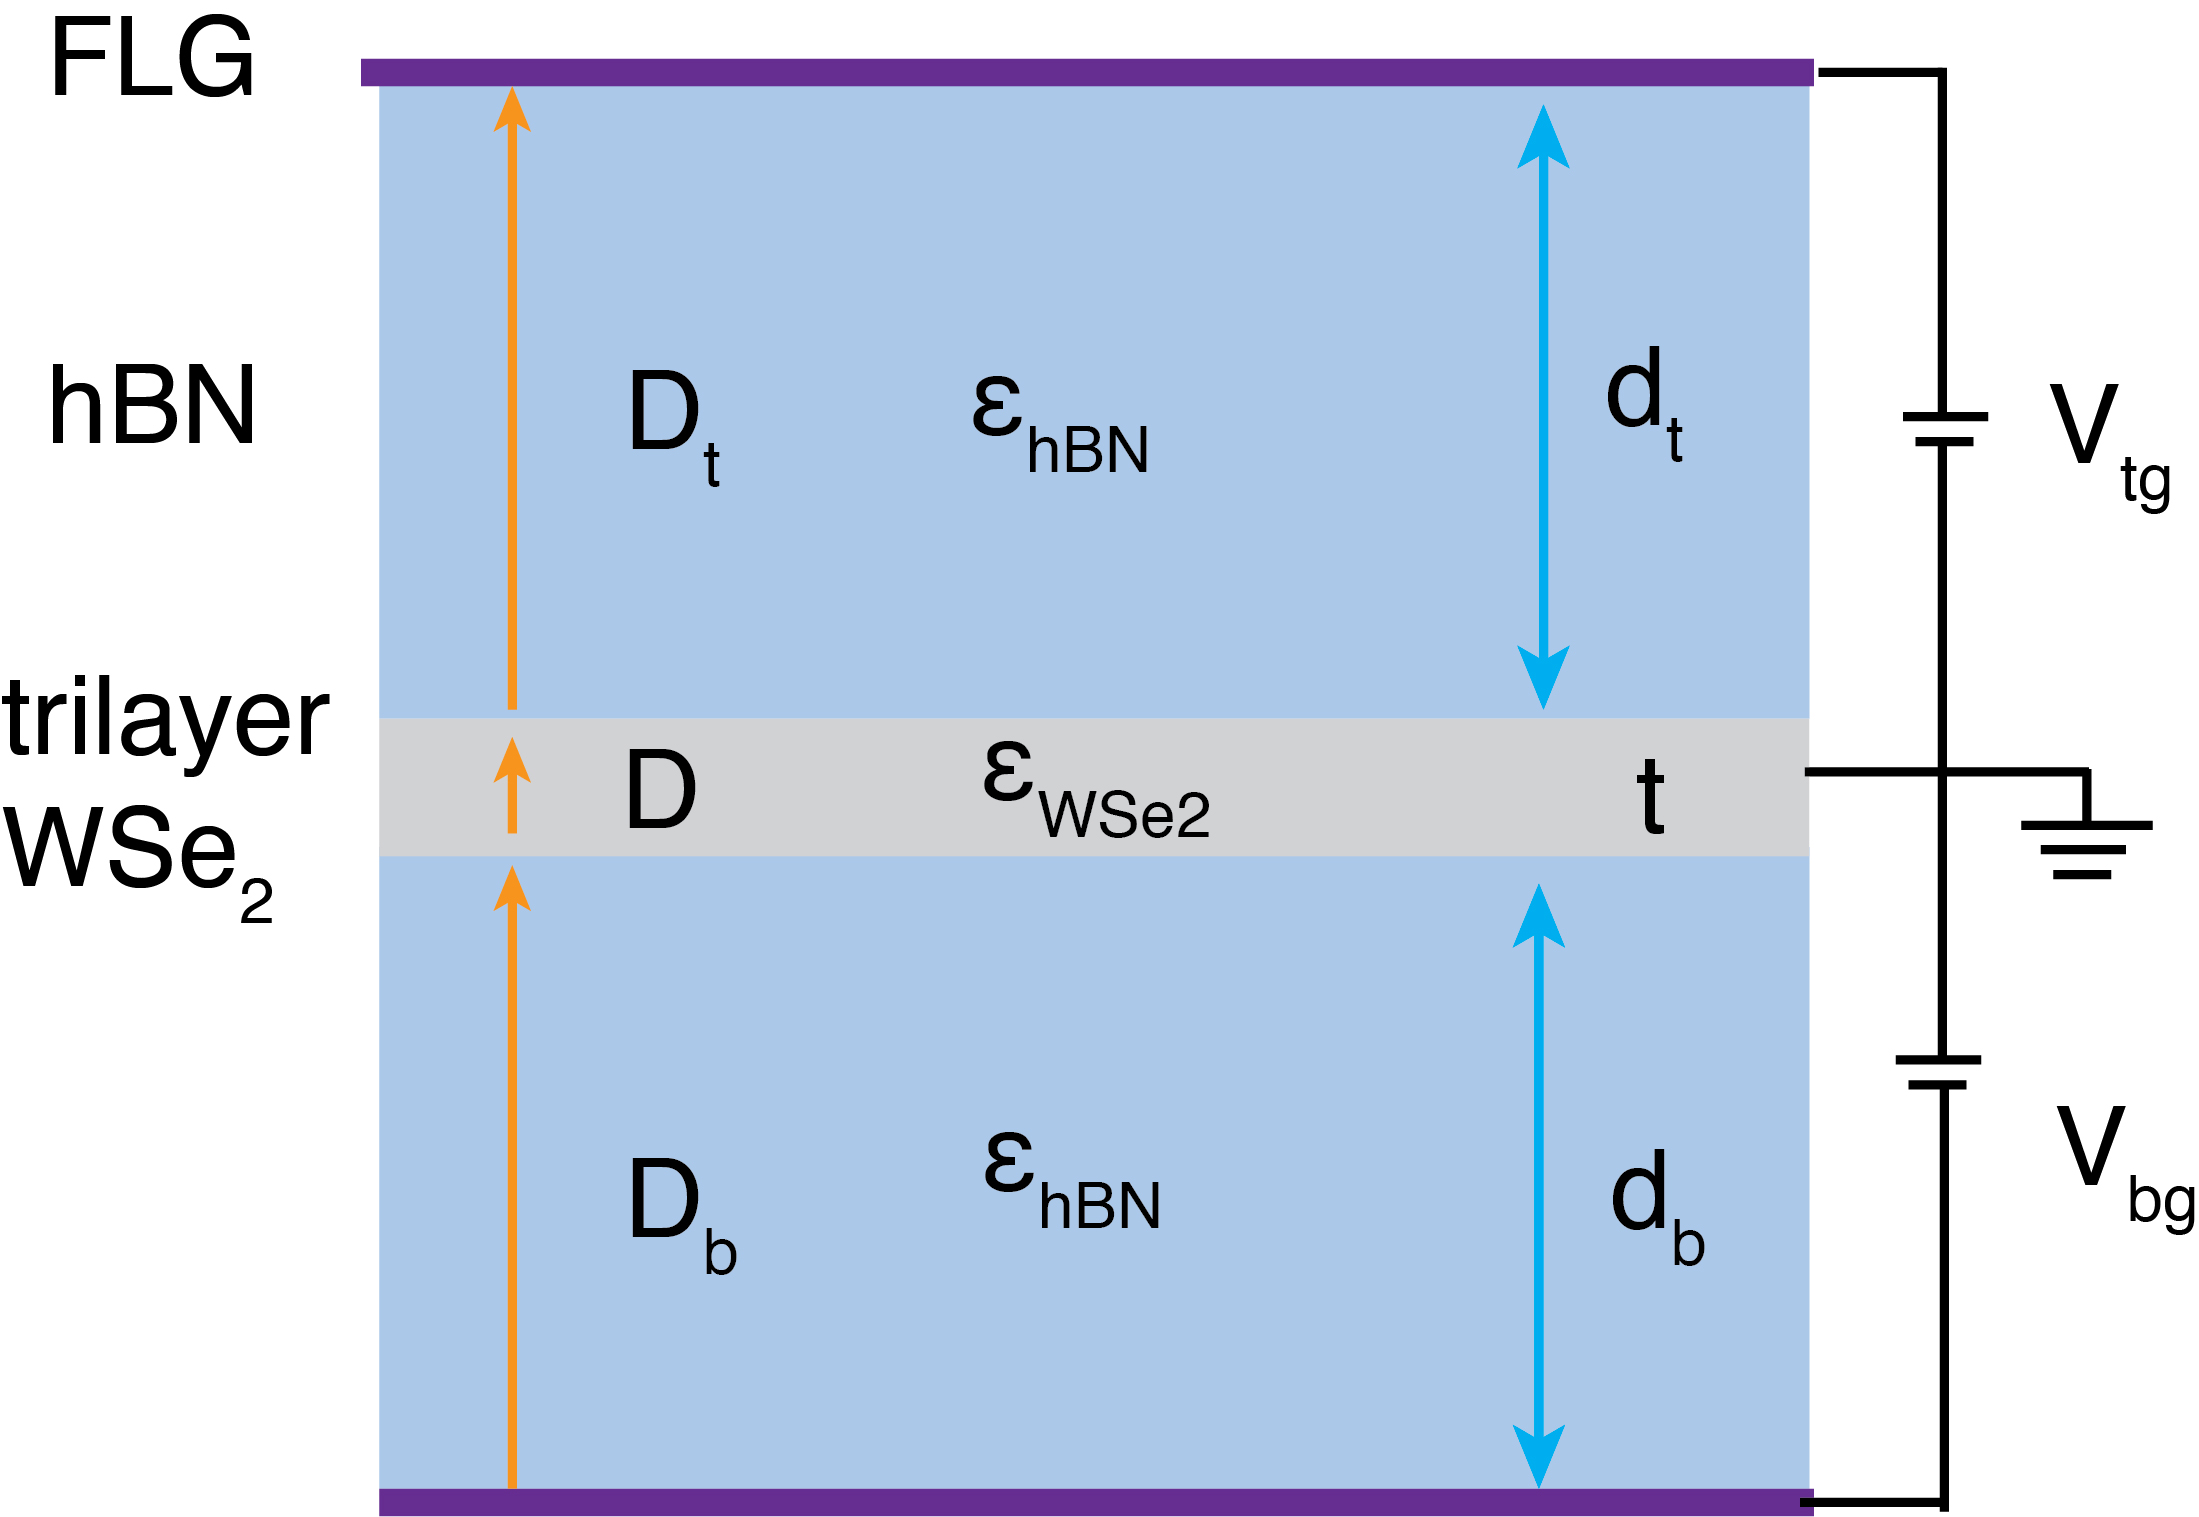
\includegraphics[width=0.45\textwidth]{Figures/C3/Fig.FET.jpg} % 
\end{center}
\caption[Schematic of the Dual-gate trilayer WSe$_2$ FET.] {\textbf{Schematic of the Dual-gate trilayer WSe$_2$ FET.}}
\label{fig.FET}
\end{figure}
\end{quote}
\renewcommand{\baselinestretch}{2}
\small\normalsize
% --------------

The TMD (here we use trilayer WSe$_2$ to keep it consistant with Chapter.5 )is modelled as the grounded sheet. 
Through the electrostatic gating, the generated displacement field $D_t$ and $D_b$ according to the applied $V_{tg}$ and $V_{bg}$ can lead to the net carrier doping in the TMD layer with the density of $n_{total}$ and the displacement filed $D_z$. 
These two parameters can be tunded independently through $V_{tg}$ and $V_{bg}$. The displacement field can be tuned as:
\begin{align}
D_T = C_{top} \bigl(V_{tg} - V^0_{tg}\bigr)  \label{eq:Dfield_t} \\ D_B = -C_{bot} \bigl(V_{bg} - V^0_{bg}\bigr)
\label{eq:Dfield_b}
\end{align} 
where the $V^0_{tg}$ and $V^0_{bg}$ are the voltage needed to compensate the initial environmental doping.
Then we can have the description of the top and bottom capacitance per unit area as:
\begin{align}
C_{top} = \frac{\epsilon_{0}\epsilon_{hBN}}{d_{t}} \label{eq:Ctop} \\
\quad  C_{bot} = \frac{\epsilon_{0}\epsilon_{hBN}}{d_{b}} \label{eq:Cbot}
\end{align} 
where the $d_{t}$ and $d_{b}$ are the thickness of the top and bottom encapsulated hBN, respectively.$\epsilon_{0}$ refers to the vacuum permittivity and .$\epsilon_{hBN}$ is the hBN dielectric constant, which we use a value of 3.7 for all the estimation. 
Now, we can obtain the electron density with the parallel capacitor model:
\begin{align}
n_{\text{total}} &= n_{top} + n_{bot} = \frac{1}{e} \left[ C_{top} \left( V_{tg} - V^{0}_{tg} \right) 
+ C_{bot} \left( V_{bg} - V^{0}_{bg} \right) \right] \label{eq:chargeQ}
\end{align}
As a result, we can calculate the total doping density inside the TMD by plug Eq.~\ref{eq:Ctop},\ref{eq:Cbot} into \ref{eq:chargeQ}, Finally, the net carrier doping density can be calculated as
\begin{equation}
n_{\text{total}} = \frac{1}{e}\,\epsilon_{0}\epsilon_{hBN} 
\left[ \frac{ V_{tg} - V^{0}_{tg} }{d_t}
     + \frac{ V_{bg} - V^{0}_{bg} }{d_b} \right]
\label{eq:ntotal}
\end{equation}
Then, we can calculate the displacement field $D$ accross the TMD induced through the gating (assuming there are no charges in TMD layer)
\begin{align}
\begin{split}
D &= \frac{1}{2} \left( D_{tg} + D_{bg} \right) \\
  &= \frac{1}{2}\,\epsilon_{0}\epsilon_{hBN} 
     \left[ \frac{ V_{tg} - V^{0}_{tg} }{d_t} 
          - \frac{ V_{bg} - V^{0}_{bg} }{d_b} \right]
\end{split}
\label{eq:Fieldtotal}
\end{align}
Finally, the applied electric field $F_z$ is calculated as:
\begin{align}
\begin{split}
F_z &= \frac{1}{2}\,\frac{\epsilon_{hBN}}{\epsilon_{TMD}}
     \left[ \frac{ V_{tg} - V^{0}_{tg} }{d_t} 
          - \frac{ V_{bg} - V^{0}_{bg} }{d_b} \right]
\end{split}
\label{eq:Efield}
\end{align}
The $\epsilon_{TMD}$ we use for trilayer WSe$_2$ is around 7 in \ref{chap5}.

\section{1D microcavity}
\label{1D microcavity}

\subsection{Transfer Matrix Method}
\label{Transfer Matrix Method}
The transfer matrix method (TMM) is a widely used approach for modeling the optical response of multilayer thin-film structures. 
In this method, each dielectric layer is treated as a homogeneous medium characterized by its refractive index and thickness. 
Light propagation through a layer is represented by a propagation (phase) matrix, while each interface between adjacent layers is described by a dynamical matrix derived from the Fresnel reflection and trans-mission coefficients. 
By multiplying the matrices of all layers, one obtains a global transfer matrix that directly relates the incident and transmitted electromagnetic field amplitudes, from which the reflectance, transmittance, and absorption spectra can be calculated.  

To illustrate the method, consider a three-medium system with refractive indices $n_0$, $n_1$, and $n_2$, where the middle film has thickness $L$ as shown in the Fig.~\ref{fig.TMM}.

%Fig.3--------------
\renewcommand{\baselinestretch}{1}
\small\normalsize
\begin{quote}
\begin{figure}
\begin{center}
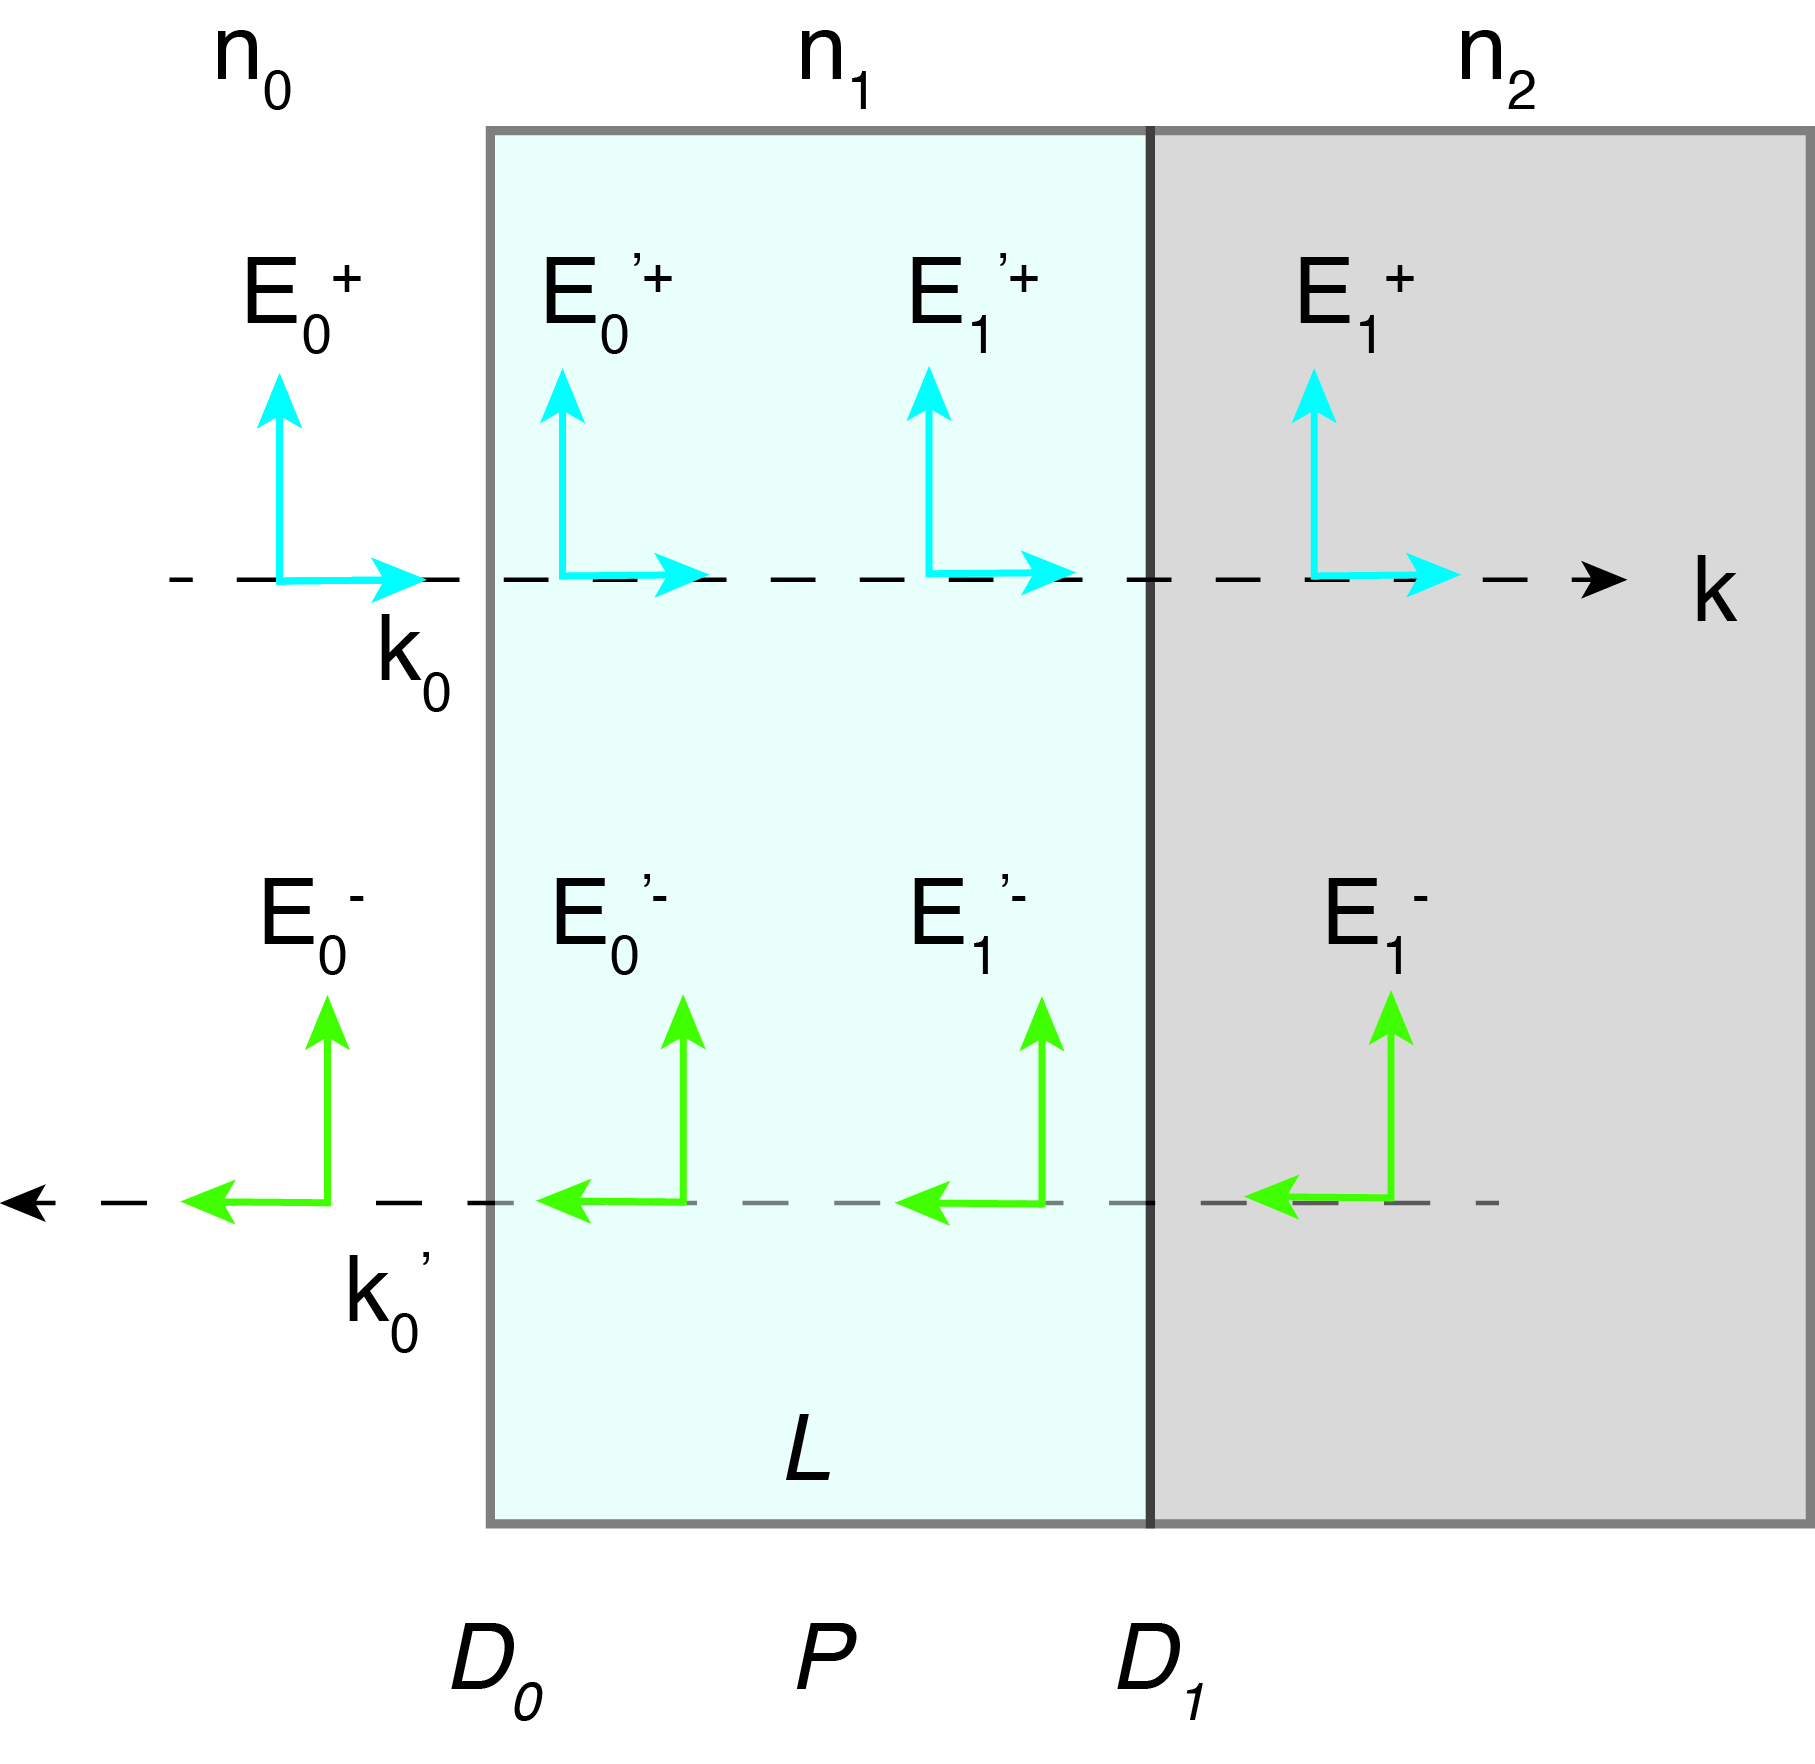
\includegraphics[width=0.4\textwidth]{Figures/C3/Fig.TMM.jpg} % 
\end{center}
\caption[Schematic of the layered structure with propagating wave's electric field and wave vector.] {Schematic of the layered structure with propagating wave's electric field and wave vector.The thickness of the dielectric materials is set as L}
\label{fig.TMM}
\end{figure}
\end{quote}
\renewcommand{\baselinestretch}{2}
\small\normalsize
% --------------

For TE (s-polarized) light, the vacuum wavenumber is $k_0 = 2\pi/\lambda$ and the longitudinal wavevector component in each medium is defined as
\begin{equation}
q_j = k_0 n_j \cos\theta_j, 
\qquad j \in \{0,1,2\},
\label{eq:q_def}
\end{equation}
with the angles $\theta_j$ constrained by Snell’s law,
\begin{equation}
n_0 \sin\theta_0 = n_1 \sin\theta_1 = n_2 \sin\theta_2.
\label{eq:snell}
\end{equation}

The electric field in each region can then be expressed as a superposition of forward- and backward-propagating plane waves:
\begin{equation}
E(x)=
\begin{cases}
E_0^{+} e^{i k_0 x} + E_0^{-} e^{-i k_0 x}, & \text{for } x<0,\\[4pt]
E_1^{+} e^{i k_1 x} + E_1^{-} e^{-i k_1 x}, & \text{for } 0<x<L,\\[4pt]
E_2^{+} e^{i k_2 (x-L)} + E_2^{-} e^{-i k_2 (x-L)}, & \text{for } x>L.
\end{cases}
\label{eq:Ex_f}
\end{equation}
By enforcing continuity of the electric field and its derivative at each interface, one obtains the Fresnel reflection and transmission amplitudes for TE polarization:
\begin{equation}
r_{ij}^{(\mathrm{TE})} = \frac{q_i - q_j}{q_i + q_j}, 
\qquad
t_{ij}^{(\mathrm{TE})} = \frac{2 q_i}{q_i + q_j}.
\label{eq:fresnel}
\end{equation}

These amplitudes are then used to construct the dynamical matrices. 
At the left interface ($n_0|n_1$) and right interface ($n_1|n_2$), the relations take the form
\begin{equation}
D_0 = \frac{1}{t_{01}}
\begin{pmatrix}
1 & r_{01} \\
r_{01} & 1
\end{pmatrix}, 
\qquad
D_1 = \frac{1}{t_{12}}
\begin{pmatrix}
1 & r_{12} \\
r_{12} & 1
\end{pmatrix}.
\label{eq:D_matrices}
\end{equation}

Propagation inside the film of thickness $L$ is described by a diagonal matrix that accounts for the phase shift $\delta = q_1 L$ of forward and backward waves:
\begin{equation}
P =
\begin{pmatrix}
e^{+i\delta} & 0 \\
0 & e^{-i\delta}
\end{pmatrix}.
\label{eq:P_matrix}
\end{equation}

The total transfer matrix of the structure is obtained by combining the interface and propagation matrices as
\begin{equation}
T = D_1 P D_0 =
\begin{pmatrix}
A & B \\
C & D
\end{pmatrix},
\qquad
\begin{pmatrix}
E_1^{+} \\
E_1^{-}
\end{pmatrix}
=
T
\begin{pmatrix}
E_0^{+} \\
E_0^{-}
\end{pmatrix}.
\label{eq:T_matrix}
\end{equation}
Explicitly, the matrix elements are
\begin{align}
A &= \frac{e^{+i\delta} + r_{12} r_{01} e^{-i\delta}}{t_{12} t_{01}}, &
B &= \frac{r_{01} e^{+i\delta} + r_{12} e^{-i\delta}}{t_{12} t_{01}}, \label{eq:AB_elements}\\[6pt]
C &= \frac{r_{12} e^{+i\delta} + r_{01} e^{-i\delta}}{t_{12} t_{01}}, &
D &= \frac{r_{12} r_{01} e^{+i\delta} + e^{-i\delta}}{t_{12} t_{01}} .
\label{eq:CD_elements}
\end{align}

Finally, the reflection and transmission amplitudes can be obtained by applying the boundary condition that no wave is incident from the right-hand side ($E_1^- = 0$). 
This leads to
\begin{equation}
r = \frac{E_0^-}{E_0^+} = -\frac{C}{D},
\qquad
t = \frac{E_1^+}{E_0^+} = \frac{\det T}{D} = \frac{q_2/q_0}{D}.
\label{eq:rt}
\end{equation}
The measurable reflectance and transmittance are then
\begin{equation}
R = |r|^2,
\qquad
T = \frac{\mathrm{Re}(q_2)}{\mathrm{Re}(q_0)} |t|^2,
\qquad
A = 1 - R - T.
\label{eq:RTA}
\end{equation}

\subsection{Distributed Bragg Reflector(DBR)}
\label{Distributed Bragg Reflector(DBR)}
A high quality-factor (Q) microcavity is essential to minimize photon losses and extend the photon lifetime, thereby enhancing the light-matter coupling strength and nonlinear interactions among polaritons. 
A Fabry–Pérot cavity composed of distributed Bragg reflectors (DBRs) offers simple, well-defined optical modes that are easy to model and measure, making it particularly suitable for polariton studies in 2D materials. 
Each DBR is formed by alternating two dielectric materials with a high refractive index contrast, with each layer thickness set to $l = \frac {\lambda}{4 n_0}$ to achieve constructive interference and high reflectivity within the stopband. 
Placing two DBRs with a separation corresponding to an optical thickness of $l_c = \frac {\lambda}{2 n_0}$ forms a resonance at $\lambda_0$.

\section{Metrology}
\label{sec:Metrology}

\subsection{PFM}
Piezoresponse Force Microscopy (PFM) is an atomic force microscopy–based technique for characterizing piezoelectric and ferroelectric materials at the nanoscale. 
In PFM, a conductive AFM tip is brought into contact with the sample surface, and an AC voltage is applied between the tip and the bottom electrode. 
The converse piezoelectric effect causes the local sample region to expand and contract at the excitation frequency, which in turn drives oscillations of the cantilever. 
The amplitude of this oscillation reflects the strength of the local piezoelectric response, while the phase indicates the polarization orientation, enabling imaging of ferroelectric domain structures with nanometer resolution.

In the conventional single-frequency implementation, the tip is typically driven near the cantilever’s contact resonance to amplify the weak electromechanical signal. 
However, the reso-nance frequency varies locally with changes in mechanical stiffness, tip–sample contact, and topography. 
Because the drive frequency is fixed, these variations lead to unstable signals, reduced sensitivity, and cross-talk with topographic features, which limits the quantitative re-liability of single-frequency PFM.

To overcome these limitations, Dual AC Resonance Tracking (DART-PFM) was developed. 
Instead of a single excitation frequency, two drive frequencies are applied on either side of the contact resonance. 
The cantilever response is demodulated at both frequencies, and the difference in amplitude serves as an error signal to track the true resonance in real time as it shifts across the sample. 
In this way, the system remains locked to resonance throughout scanning, ensuring maximum sensitivity and stable phase contrast. 
DART-PFM thereby combines the resonance amplification of single-frequency PFM with robust frequency tracking, yielding higher signal-to-noise ratio and quantitative reproducibility. 
It is particularly powerful for imaging complex domain structures and for performing switching spectroscopy, where consistent sensitivity during bias sweeps is critical.

In this work, the PFM characterization is performed with DART- PFM (Dual AC Resonance Tracking Piezo Force Microscopy) mode by Oxford Asylum Cypher ES at room temperature. 
We used Ti/Ir coated conductive cantilever probes with resonance frequency of 75 kHz and a spring constant of 2.8 N/m (ASYELEC-01-R2).
We applied an AC bias with a driving amplitude of 3 V between the tip and the sample to generate an electric field in the vertical direction. 
This field induces a piezoelectric response in the sample, which is detected by monitoring the tip deflection through the laser diode. 
PFM images are obtained with a scan rate of 1Hz and a $0^{\circ}$ scan angle.
This setup enables reliable imaging of ferroelectric domains and polarization switching in thin films and emerging low-dimensional systems, providing both structural and functional information at the nanoscale.

\section{Optical Spectroscopy}
\label{sec:Optical Spectroscopy}
Optical spectroscopy is the main method for characterizing the excitonic behavior in TMD system. 

\subsection{Real- and Fourier space confocal microscopy}
PL(Photoluminescent) and reflectance measurement are the main optical methods we apply to study the emission and absorption property of the TMD materials.

PL probes the radiative recombination of photoexcited carriers and excitons in semiconductor system.
An above-gap pump creates electron–hole pairs that rapidly relax to band-edge states; bound excitons (and, when doped, trions/polaron states) then recombine and emit at characteristic energies. 
Reflectance spectroscopy is a widely used technique to probe the excited staes of the solid-state materials. 
It provides information about cavity modes, excitonic resonances, and interference effects in thin films and heterostructures.  
In all the reflectance measurement performed in this thesis, the reflectance spectrum of the TMD region is normalized with the reference region(hBN or gold). 
This normalized reflectance, expressed as the $\Delta R = R_{Sample}/R_{bg}$, highlights spectral features associated with the material and suppresses background contributions from the substrate or optical components.

A shematic of the optical setup we used in the thesis is shown in the Figure~\ref{fig.OS}. 
For excitonic study(Chapter 4,5), we primaryly used the collection path shared with the excitation path with a Galvo mirror system. 
This enables rapid acquisition of spatially resolved optical maps and accessing each spot's spectrum on the sample without moving the stage.
A 4f lens system(L5 and L6) after the galvo mirrors relays the beam so that angular deflections at the galvo are mapped to the back focal plane of the objective. 
This keeps the excitation spot fixed on the sample while allowing precise beam scanning without distortion.
At the collection path, a 10 X objective focues the beam onto the single mode fiber. The fiber core with a mode field diameter of 4 $\mu m$ serve as confocal pinhole.

For cavity and polariton study(Chapter 6), the Fourier-space imaging is needed to explore the polariton dispersion. 
In contrast to the real-space imaging, Fourier-space imaging first collects lights accross the whole sample with different reflected/emitted angle and then focues the beam to the entrance slit of the spectrometer(shown in the left part of the schematic).

For cavity and polariton characterization, k-space imaging is needed to study their dispersion relationship in momentum (photon energy vs. the wavevector). 
This is based on capturing the angular distribution of the reflected light.
In our set up, we directly image the back focal plane (Fourier plane) of the objective lens to the detector through the lenses combination (relay lens L1,L3 and focus lens L4)
In this configuration, light emitted at a specific angle is focused to a unique point on the spectrometer by lens L4, regardless of where it originated on the sample surface. 
As a result, to enhance data quality, measurements were restricted to a single selected spot by an x-y adjustable pinhole at the real space focal point, thereby minimizing the influence of sample inhomogeneity.

To calibrate the corresponding in plane momentum $k_{||}$ for each y pixel on the CCD sensor for the angle-resolved measurement, we need to first calculate the corresponded beam angle for each pixel on the y axis. 
The maximum collection angle depends on the objective NA as:

\begin{equation}
\text{NA} = n \cdot \sin\theta 
\label{eq:NA}
\end{equation}

where $i$ is the pixel index, $i_0 = N/2$ is the center pixel, and $N$ is the total number of pixels along the $y$-axis of the CCD.  

The corresponding in-plane momentum $k_{\parallel}$ is then given by
\begin{equation}
k_{\parallel} = \frac{2\pi}{\lambda} \cdot \sin\phi .
\label{eq:k_parallel}
\end{equation}

All the above optical measurements were carried out in attoDRY 800 closed-cycle cryostat (operated near 4 K).
An apochromatic objective inside the cryostat (NA = 0.82) focuses the 635 nm diode laser to a diffraction-limited spot $(\mathrm{FWHM}\approx 0.51\,\lambda/\mathrm{NA}\approx 0.4~\mu\mathrm{m}\ \text{at}\ 635~\mathrm{nm})$ and collects the emission with a free-space to fiber coupler. The signal is then dispersed by a Horiba iHR320 spectrometer (300 lines/mm grating) and detected on a Synapse-Plus visible CCD. 
The single mode fiber core with a size of 4 $\mu m$ serve as confocal pinhole.


%Fig.4--------------
\renewcommand{\baselinestretch}{1}
\small\normalsize
\begin{quote}
\begin{figure}
\begin{center}
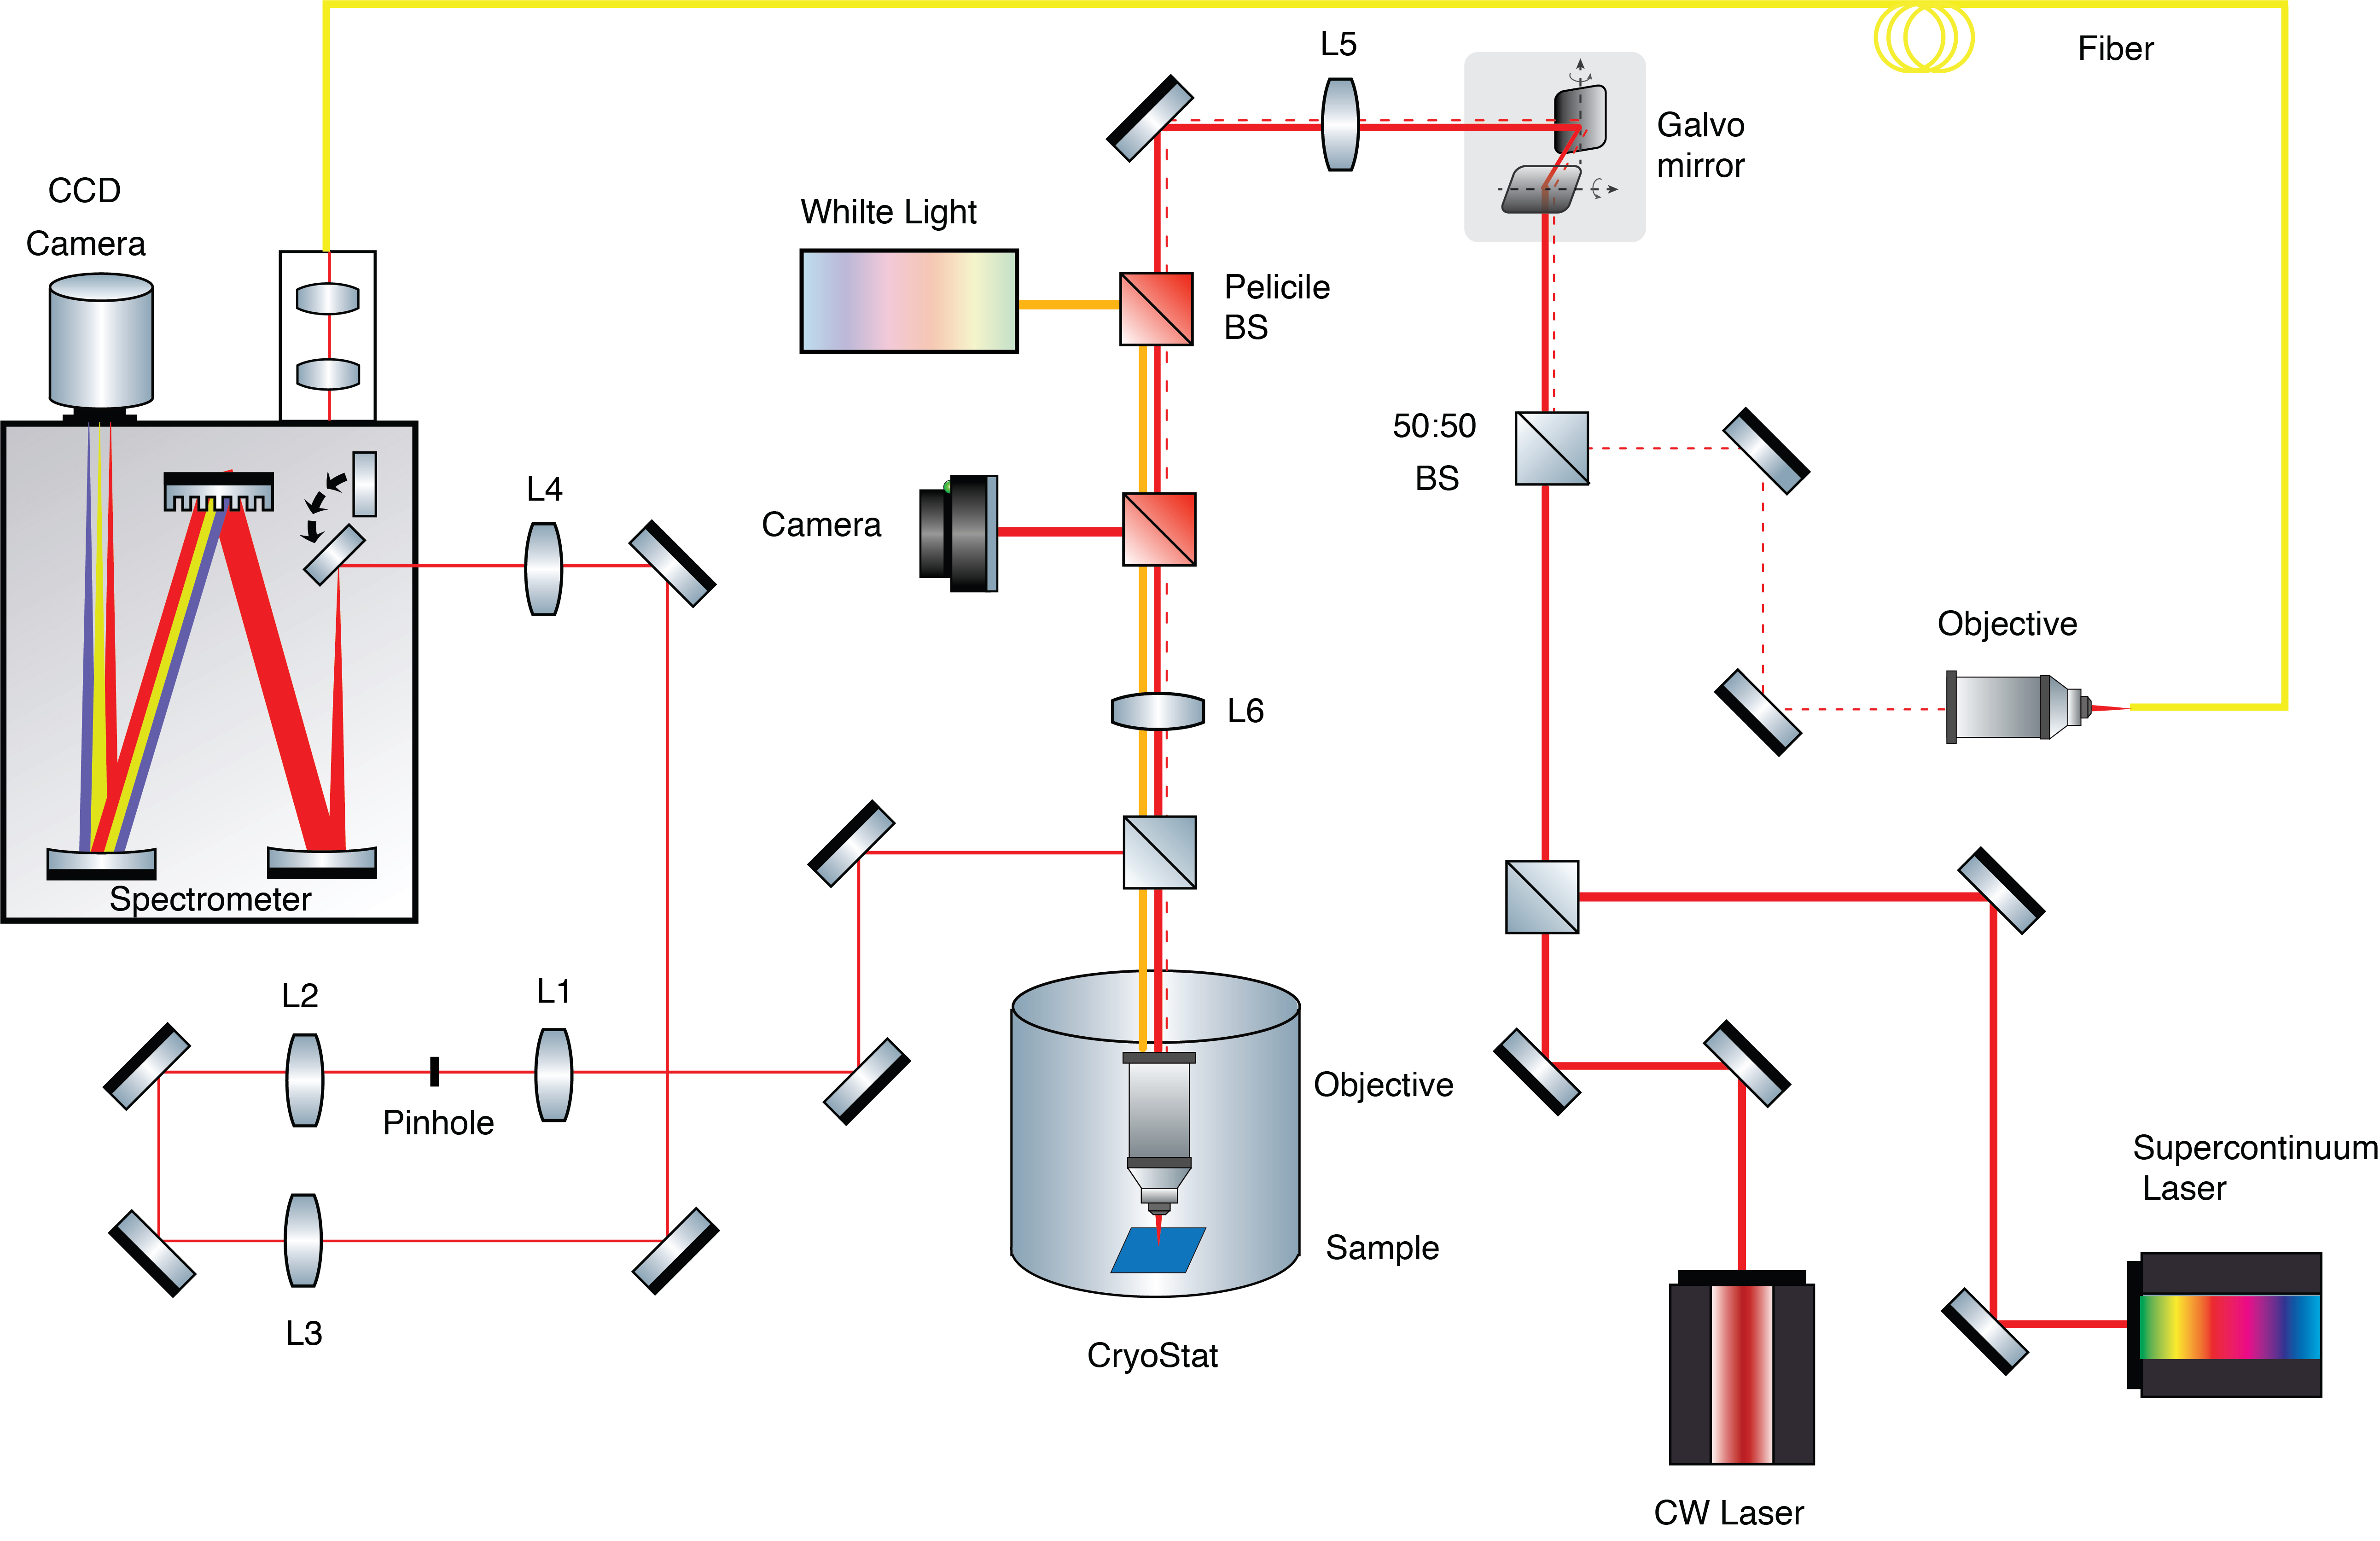
\includegraphics[width=1\textwidth]{Figures/C3/Fig.Setup.jpg} % 
\end{center}
\caption[Real-space and Fourier-space spectroscopy experimental setup.] {\textbf{Real-space and Fourier-space spectroscopy experimental setup.} L1 and L3(flip) are the Fourier plane relay lens. The distance before L1 to the objective is set as $2f_1$.  The distance between L1 and L3 is set as $2f_1+f_3$. L1 and L2(flip) are the real plane relay lens.The distance between L1 and L2 is set as $2f_1+f_2$.The pinhole is set at center between L1 and L2. L4 is the imaging lens for the spectrometer.}
\label{fig.OS}
\end{figure}
\end{quote}
\renewcommand{\baselinestretch}{2}
\small\normalsize
% --------------